\documentclass{beamer}

\usepackage{listings}
\usepackage{color}

% Code colorature
\definecolor{paszt}{RGB}{252,252,252}
\definecolor{keret}{RGB}{220,220,220}
\lstset{
backgroundcolor=\color{paszt},
% showlines=true,
framexleftmargin=4mm,
framexrightmargin=4mm,
framextopmargin=2mm,
framexbottommargin=2mm,
frameround=tttt,
frame=trbl,
rulecolor=\color{keret}
}

\usetheme{Copenhagen}
\useinnertheme{rectangles}

%\usetheme{Berlin}
%\usecolortheme{beaver}
%\useinnertheme{beaver}

% ---- Mongo theme ----
%\definecolor{light-background}{RGB}{210,250,170}
%\definecolor{dark-background}{RGB}{128,92,64}
%\usecolortheme[RGB={220,250,180}]{structure}

% ---- Vanilla theme ----
% \definecolor{light-background}{RGB}{250,250,190}
% \definecolor{dark-background}{RGB}{128,92,64}
% \usecolortheme[RGB={210, 210, 140}]{structure}

% ---- Blue theme ----
\definecolor{light-background}{RGB}{200,220,240}
\definecolor{dark-background}{RGB}{100,110,120}
\usecolortheme[RGB={180, 200, 230}]{structure}

% ---- Green theme ----
%\definecolor{light-background}{RGB}{229,237,204}
%\definecolor{dark-background}{RGB}{156,163,140}
%\usecolortheme[RGB={180, 210, 150}]{structure}

%\setbeamercolor{palette primary}{fg=black, bg=light-background}
%\setbeamercolor{palette quaternary}{fg=white,bg=dark-background}

\setbeamercolor{title}{fg=black}
\setbeamercolor{frametitle}{fg=black}

% Set font
%\usefonttheme{structurebold}

\frenchspacing

% Language packages
\usepackage[utf8]{inputenc}
\usepackage[T1]{fontenc}
\usepackage[magyar]{babel}

% AMS
\usepackage{amssymb,amsmath}

% Graphic packages
\usepackage{graphicx}

% Syntax highlighting
\usepackage{listings}
\usepackage{rust}
\usepackage{cpp}

%\usepackage{tikz}

%\begin{figure}[htb]
%\begin{center}
%	\includegraphics[scale=0.4]{ps_times.png}
%\end{center}
%\end{figure}

% ==============
\begin{document}
% ==============

\title[Numerikus számítások megvalósítása Rust programozási nyelven]{
{\Large Numerikus számítások megvalósítása \\ Rust programozási nyelven}
}
\author[László Bence]{\Large László Bence}
\date{Miskolci Egyetem, 2019. június 17.}

% --------------------
% Title page
\frame{\titlepage}

% --------------------
\begin{frame}[fragile]
\frametitle{Motiváció, célkitűzések}

\begin{itemize}
\item A numerikus számításokat jellemzően C és Fortran nyelven implementálják.
\item Hatékonyak, de nem tekinthetők modern eszközöknek.
\item A dolgozat célja, hogy összehasonlítsa a C és Rust teljesítményét elsősorban futási idő szempontjából.
\item Áttekint néhány gyakran előforduló numerikus problémát.
\item Azt vizsgálja, hogy a Rust alternatíva-e számításigényes alkalmazások készítéséhez.
\end{itemize}

\end{frame}

% --------------------
\begin{frame}[fragile]
\frametitle{A Rust programozási nyelv [1]}

\begin{itemize}
\item Hatékony, biztonságos memóriamodell
\item Tesztek, dokumentálás nyelvi szinten elérhető
\item Szabványos csomagkezelő és build eszköz (\texttt{cargo})
\end{itemize}

\begin{figure}[htb]
\begin{center}
	
\includegraphics[scale=0.25]{images/rust.png}
\end{center}
\end{figure}

\end{frame}

% --------------------
\begin{frame}[fragile]
\frametitle{Futási idő mérése}

GNU Time parancs [2]
\begin{cpp}
time -f %E_%P_%M
\end{cpp}

\medskip

Rust, \texttt{coarsetime} függvénykönyvtár [3]

\medskip

\begin{itemize}
\item A bemenetek egyenletes eloszlás szerint generált lebegőpontos értékek.
\item A számítások futási idejébe a bemenetek generálása nem számít bele.
\end{itemize}

\medskip

A numerikus integráláshoz használt határozott integrál:
\[
F(x) = \int_0^{40} \! x^2 - 1 \; \mathrm{d}x.
\]

\end{frame}

% --------------------
\begin{frame}[fragile]
\frametitle{Fordítók és beállításaik}

GCC 8.2.1

\begin{cpp}
gcc -O3 sample.c -o sample
\end{cpp}

\medskip

CLang 8.0.0

\begin{cpp}
clang -O3 sample.c -o sample
\end{cpp}

\medskip

Rust 1.33
\begin{cpp}
rustc -C --opt-level=3 sample.rs -o sample
\end{cpp}

\end{frame}

% --------------------
\begin{frame}[fragile]
\frametitle{Numerikus módszerek}

A vizsgált numerikus módszerek [4]:
\begin{itemize}
\item Numerikus integrálás: trapéz szabály, Simpson formula,
\item Rendezés: kupacrendezés, Shell rendezés, gyorsrendezés,
\item Lineáris interpoláció.
\end{itemize}

\bigskip

Minden módszer esetében:
\begin{itemize}
\item Rövid matematikai bevezetés,
\item C nyelvű referencia-implementáció,
\item Rust nyelvű implementáció,
\item Futási idők, tárigény összehasonlítása.
\end{itemize}

\end{frame}

% --------------------
\begin{frame}[fragile]
\frametitle{Numerikus integrálás}

\begin{itemize}
\item Trapéz szabály, Iteratív trapéz szabály, Simpson formula
\end{itemize}

\begin{figure}[htb]
\begin{center}
	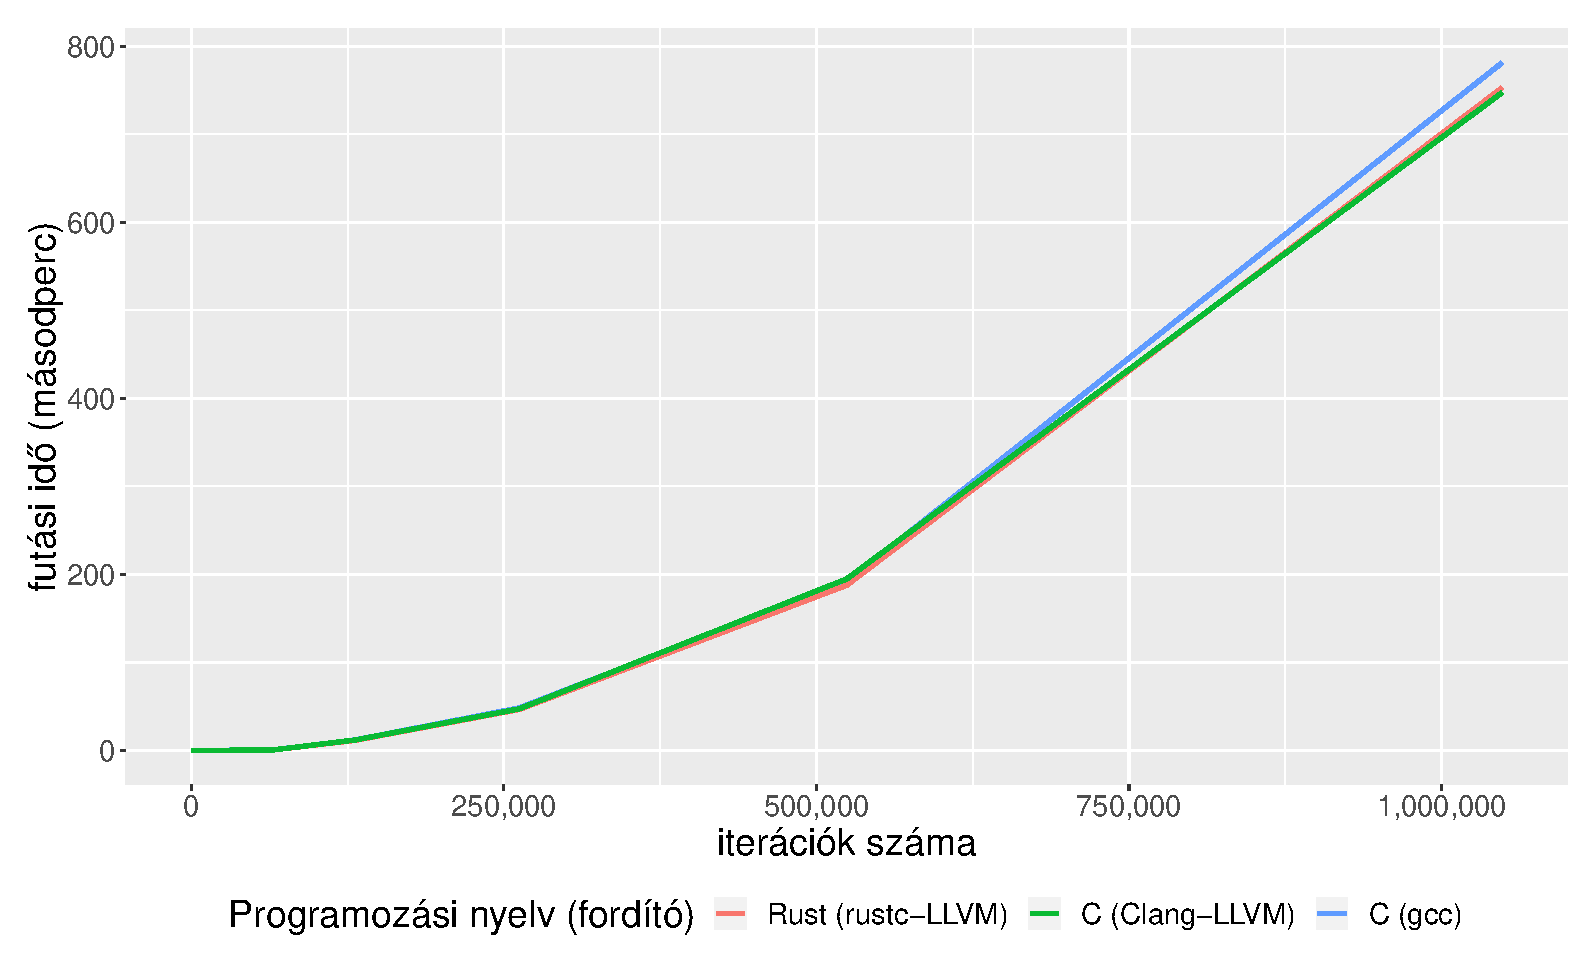
\includegraphics[scale=0.4]{images/simpsons_rule_run.eps}
\end{center}
\end{figure}

\end{frame}

% --------------------
\begin{frame}[fragile]
\frametitle{Rendezés - Kupac rendezés futási ideje}

\begin{figure}[htb]
\begin{center}
	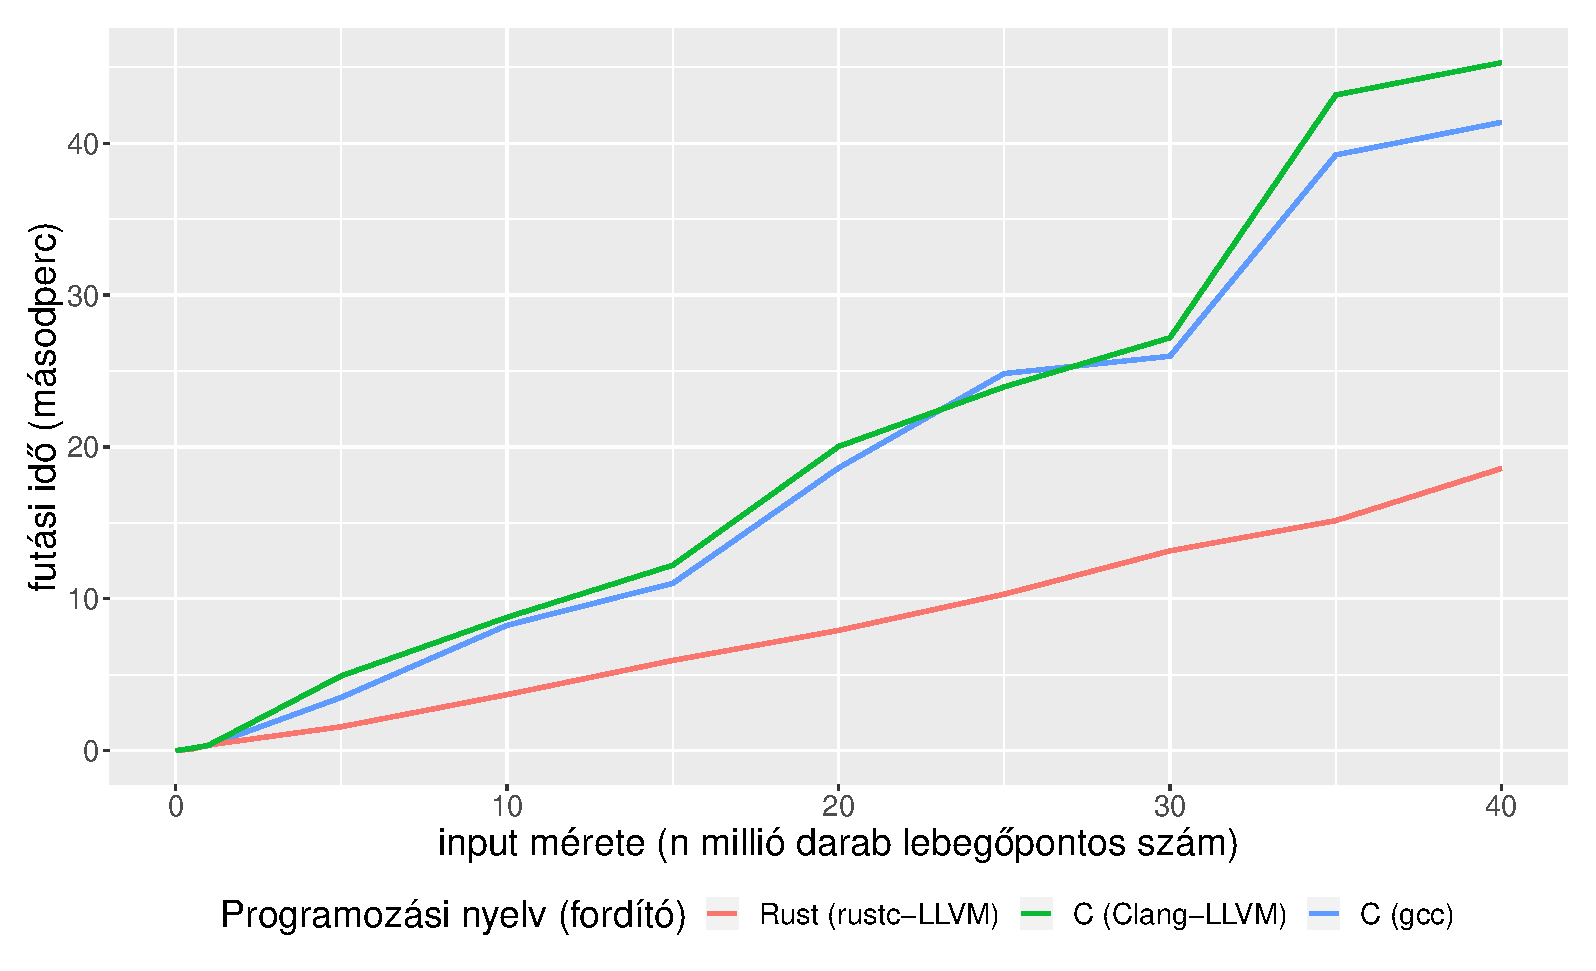
\includegraphics[scale=0.4]{images/heap_sort_run_without_read.eps}
\end{center}
\end{figure}

\end{frame}

% --------------------
\begin{frame}[fragile]
\frametitle{Rendezés - Kupac rendezés memóriaigénye}

\begin{figure}[htb]
\begin{center}
	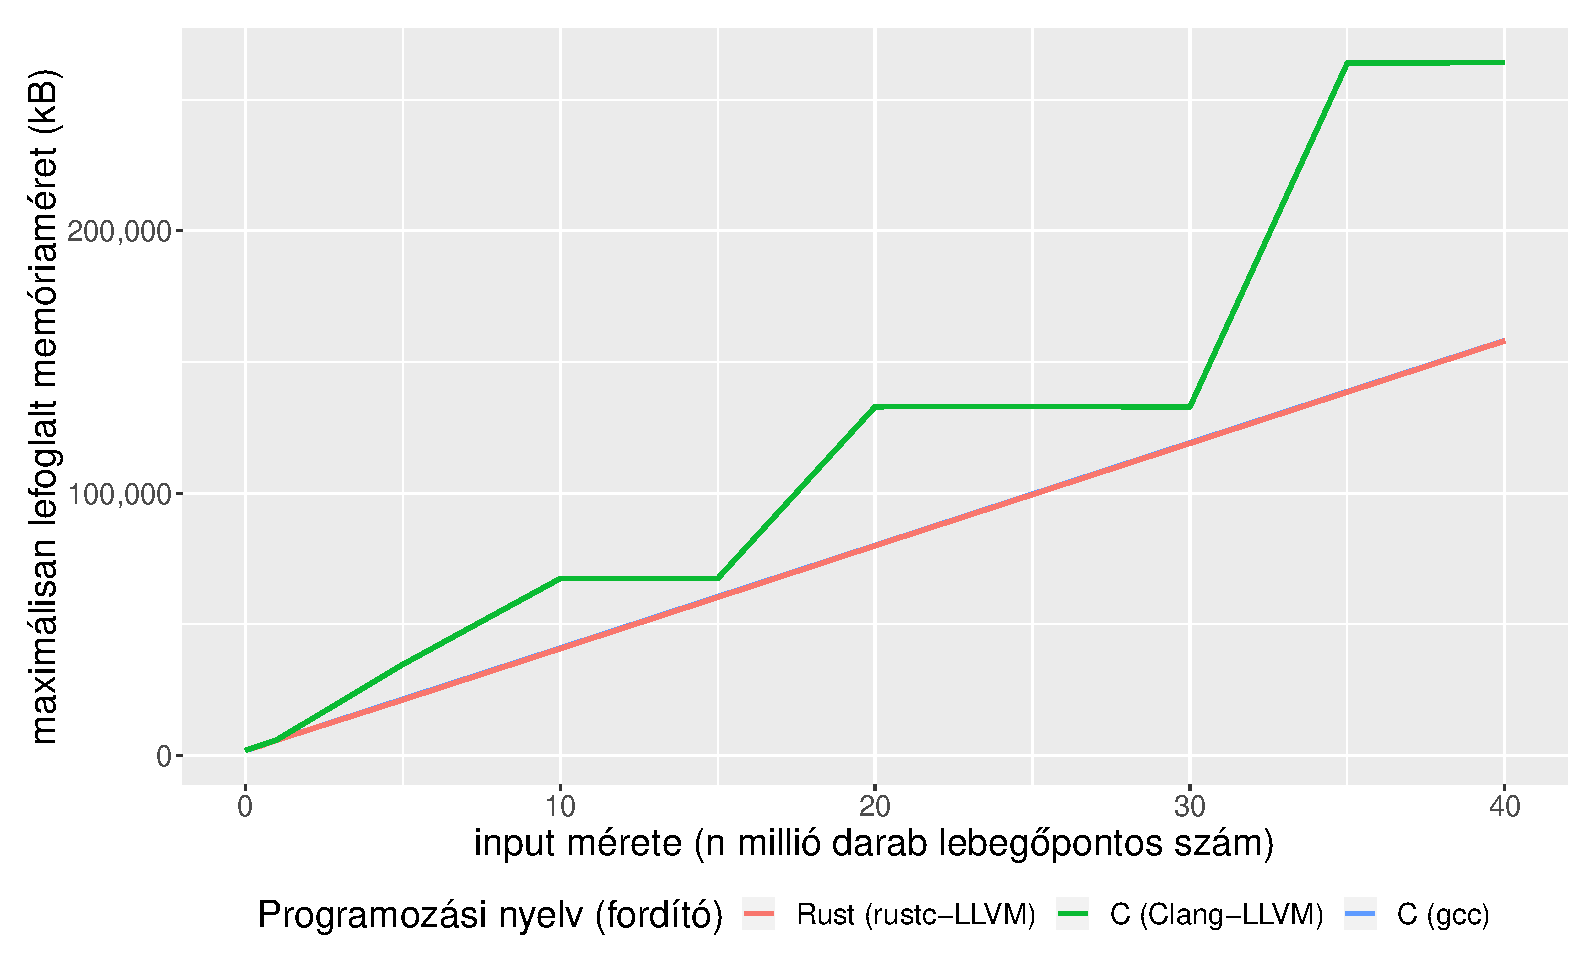
\includegraphics[scale=0.4]{images/heap_sort_memory.eps}
\end{center}
\end{figure}

\end{frame}

% --------------------
\begin{frame}[fragile]
\frametitle{Rendezés - Shell rendezés futási ideje}

\begin{figure}[htb]
\begin{center}
	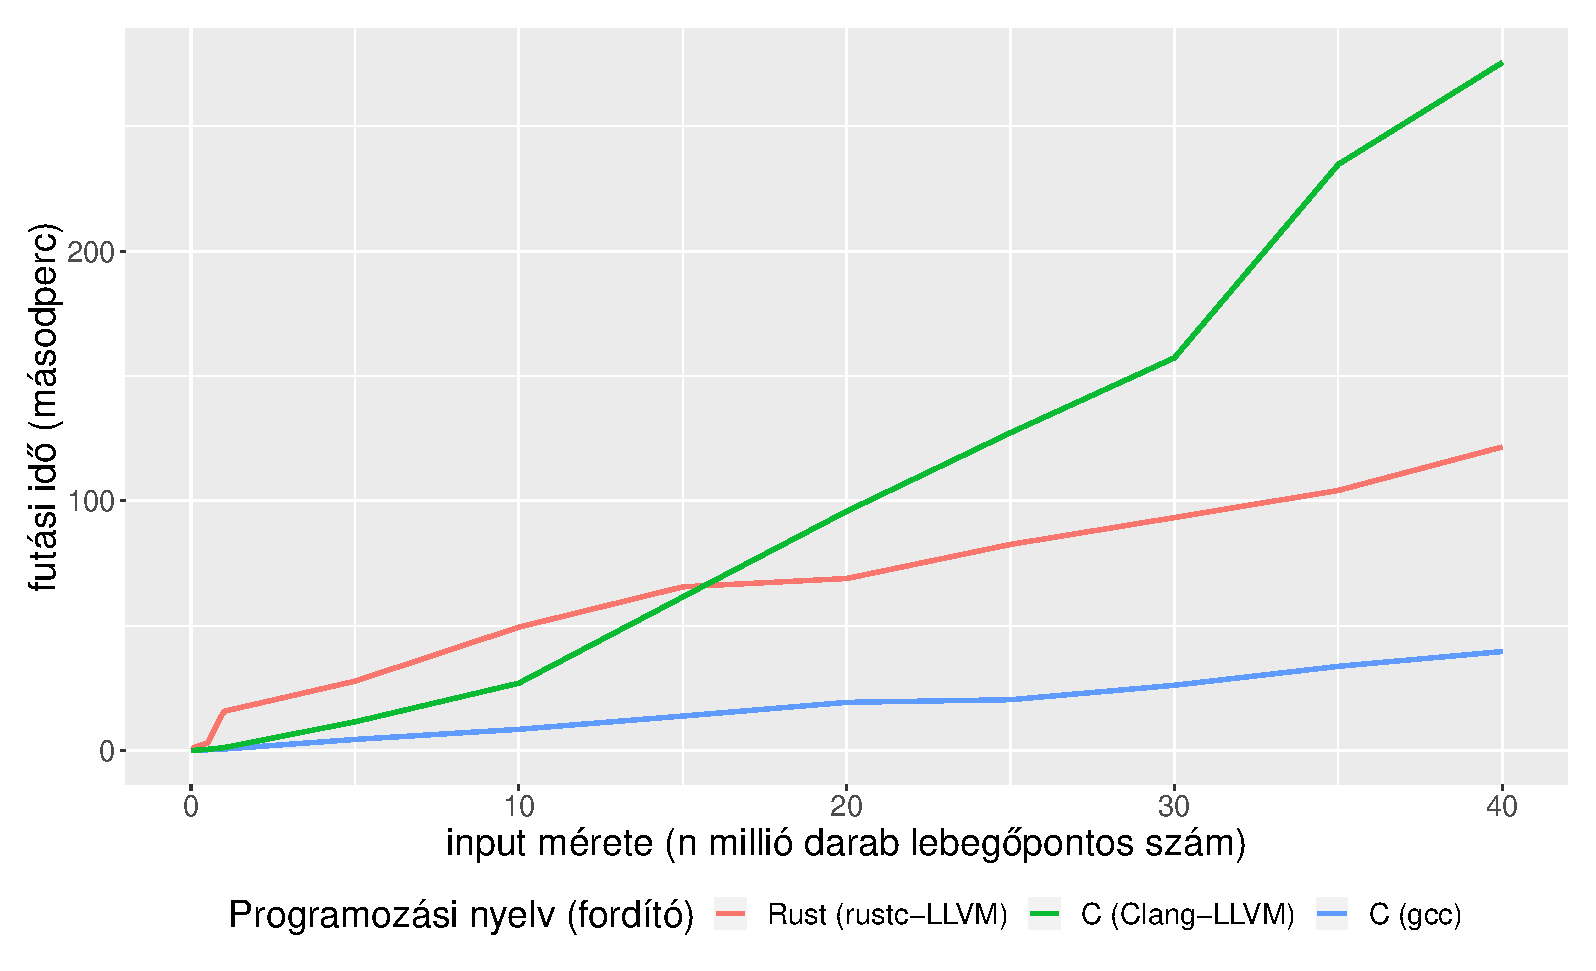
\includegraphics[scale=0.4]{images/shells_sort_run.eps}
\end{center}
\end{figure}

\end{frame}

% --------------------
\begin{frame}[fragile]
\frametitle{Rendezés - Gyorsrendezés}

\begin{figure}[htb]
\begin{center}
	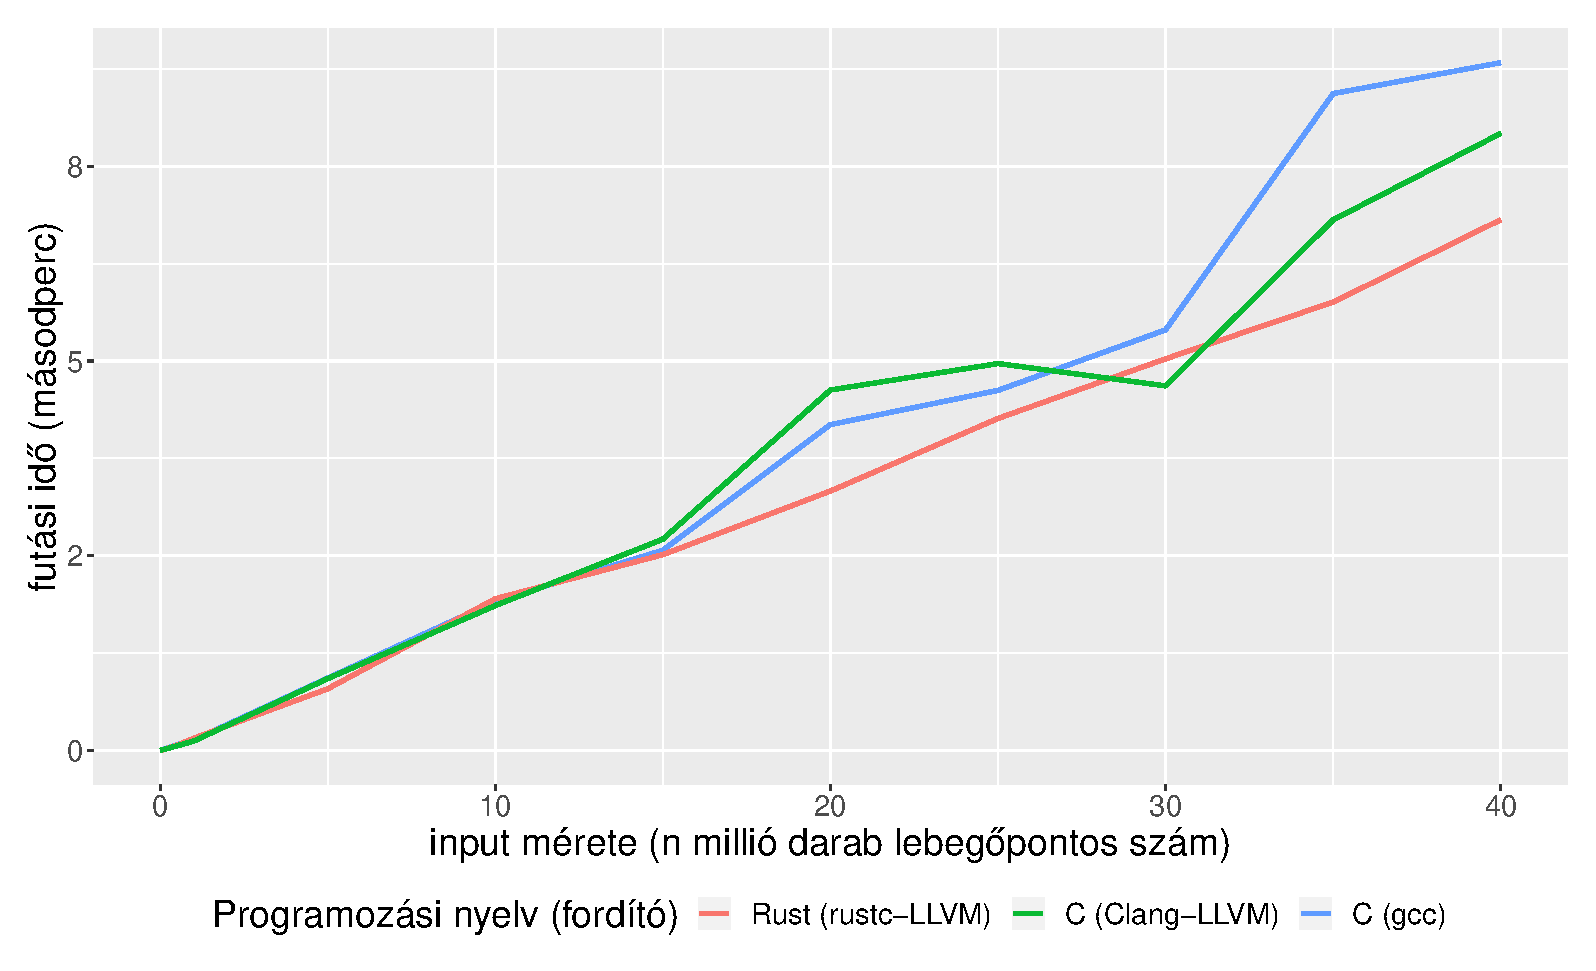
\includegraphics[scale=0.4]{images/quicksort_run_without_read.eps}
\end{center}
\end{figure}

\end{frame}

% --------------------
\begin{frame}[fragile]
\frametitle{Lineáris interpoláció futási ideje}

\begin{figure}[htb]
\begin{center}
	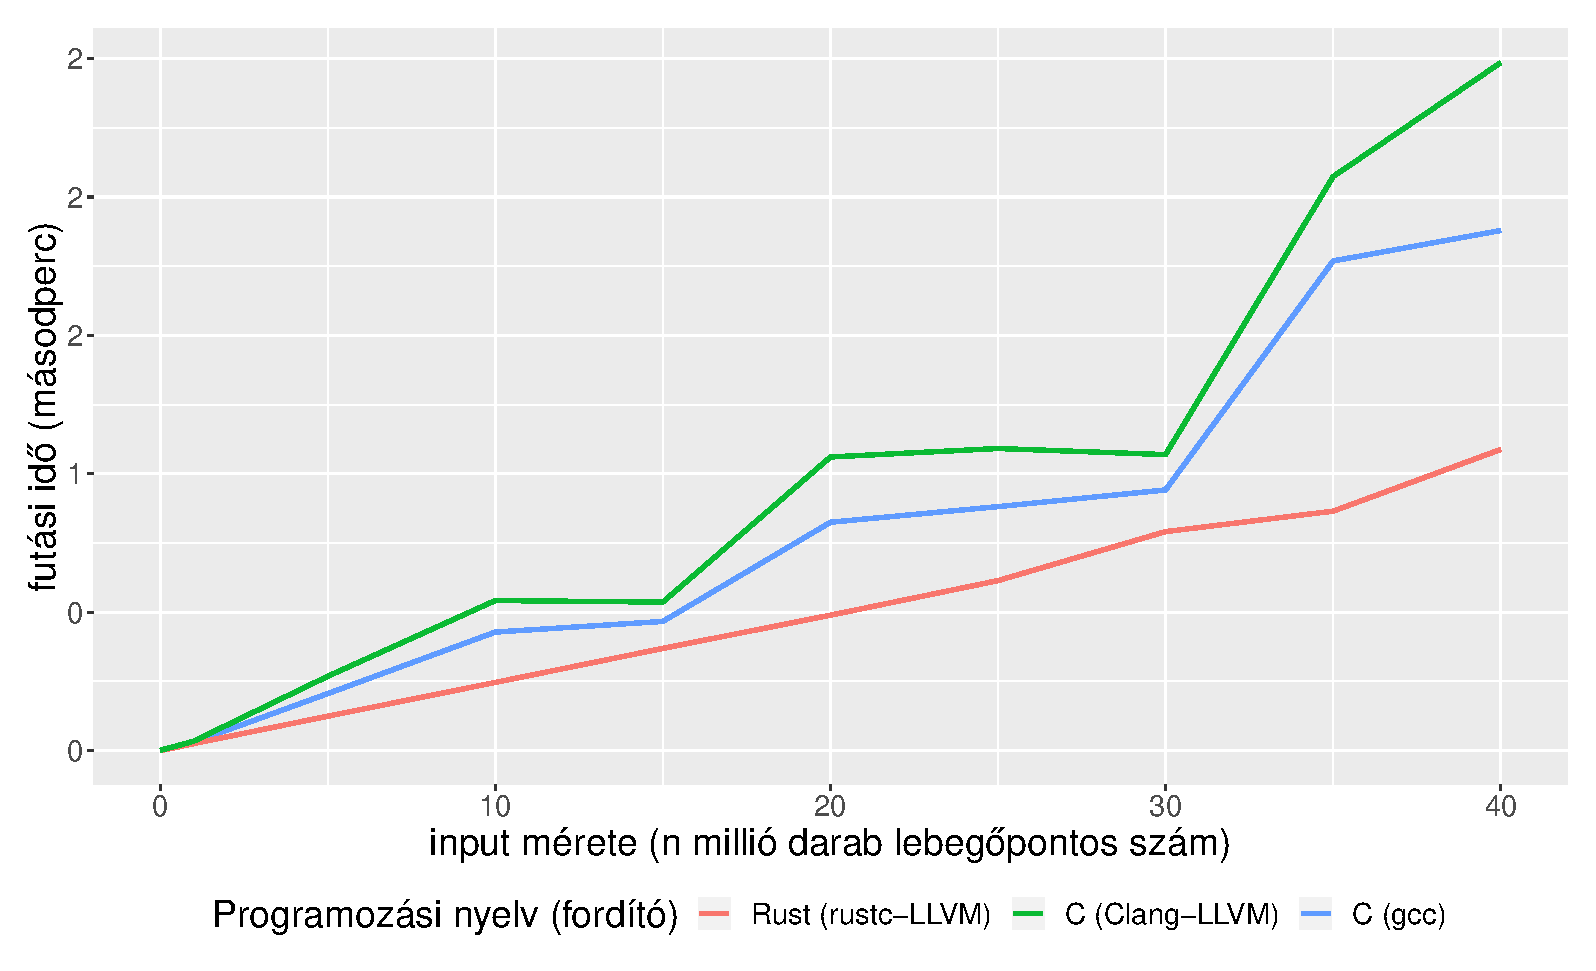
\includegraphics[scale=0.4]{images/linear_interpolation_run_without_read.eps}
\end{center}
\end{figure}

\end{frame}

% --------------------
\begin{frame}[fragile]
\frametitle{Összegzés}

\emph{A dolgozat eredményei alapján megállapítható, hogy a Rust nyelv alkalmas numerikus módszerek hatékony implementálására.}

\vskip 8mm

\textbf{További vizsgálati lehetőségek}
\begin{itemize}
\item Gyakorlatban előforduló további számítási módszerek összehasonlítása.
\item Biztonságos memóriakezelésből eredő számítási idők vizsgálata.
\item Az egyes fordítók működőséből származó különbségek, azok javítási lehetőségeinek elemzése.
\end{itemize}

\end{frame}

% --------------------
\begin{frame}[fragile]
\frametitle{Hivatkozások}

\begin{itemize}

\item[1] Klabnik, Steve, and Carol Nichols. \\
\emph{The Rust Programming Language}.
No Starch Press, 2018.

\item[2] GNU Time, hivatalos weboldal, \texttt{https://www.gnu.org/software/time}, \\
Internet, 2019.

\item[3] coarsetime, dokumentáció, \texttt{https://docs.rs/coarsetime/0.1.11/coarsetime}, Internet, 2019.

\item[4] William H. Press, Saul A. Teukolsky, William T. Vetterling, Brian P. Flannery: \emph{Numerical Recipes The Art of Scientific Computing Third Edition}. \\
Cambridge University Press, 2007.

\end{itemize}

\end{frame}

% --------------------
\begin{frame}[fragile]
    \frametitle{\ }

\begin{center}
\huge \textbf{Köszönöm szépen a figyelmet!}
\end{center}

\end{frame}

\end{document}
